\documentclass[12pt]{article}

\newcommand\floor[1]{\lfloor#1\rfloor}
\newcommand\ceil[1]{\lceil#1\rceil}

\usepackage{amsmath}
\usepackage[super]{nth}
\usepackage[utf8]{inputenc}
\usepackage[T1]{fontenc}
\usepackage{textcomp}
\usepackage{gensymb}
\usepackage{graphicx}

\pagenumbering{arabic}

\begin{document}
\title{Music Generation in ArtToMusic}
\date{February 22, 2017}
\author{Rafael De Smet}

\maketitle

\section{Music Generation}

With the help of the library Beads\footnote{http://www.beadsproject.net/}, the music is generated based on the graphical analysis. This library is just a helpful tool to produce sounds. It doesn't know anything about (good) musical patterns, rhythm or harmony. The only thing it does is generate a sounds, which is determined earlier on by the graphical analysis.

\subsection{Rhythm And Harmony}
An integral part of music is the rhythm So I decided to use the edges of the image to determine the rhythm of the music.
This is a work in progress. Later the entropy of the analysis of an image will be added to this determination.
\newline
\newline
Without a melody, there is no music. Any melody of a song is based on the rules of harmony, which notes sound good when played together, which don't? Which notes make up a chord? These kind of rules are the subject of harmony.
\newline
\newline
The program works with premade chord progressions. These are enumerations of a number of chords in a certain order which creates a melody. For example, the chord progression I-II-V-I is very familiar once you hear it. This means we play the first chord of the key we are in, then the second, then the fifth and the first one to end.
\newline
\newline
Based on how much of certain colors there are in the image we are analysing, we choose a different chord progression to work with. If there is a lot of red in the image, the program chooses the I-II-V-I progression, for instance. Other dominant colors lead to other chord progressions.

\subsection{Comparison of music generation techniques}

\subsubsection{Beads}
As mentioned before is the Beads library, developed by Ollie Bown with the support of the university of Melbourne, a very handy tool to generate music. Beads uses the concept of unit generators (UGs) as the core of the library. As described by Evan Merz, the author of \textit{Sonifying Processing: The Beads Tutorial}, a unit generator is a ``building block of the audio signal''.  One unit generator takes care of one function in the generation of music. 

A simple example of a unit generator is a guitar players distortion pedal. The clean signal of his guitar enters the generator and a distorted version of the signal is produced. Beads works as a series of unit generators (or guitar pedals).
\newline
\newline
The Beads library has multiple of these UGs, such as an envelope filter, a gain, a waveplayer, etc. The most important UG is the AudioContext. This is the main UG where every other UG plugs into. Without this there is no music but it doesn't create any sound by itself, it just acts as a connection to the computer's hardware. The audio comes from other UGs.
\newline
\newline
Beads has two main ways of creating audio.

\paragraph{Samples}

You can load multiple samples in to use later on. These samples can be anything you wish and have to be on your machine to be able to load them in the program. Once you have found the file and loaded it in via the SamplePlayer, you can use it exactly the same as any other UG, connect it to the Gain UG to determine the volume or pass it through an EnvelopeFilter, etc.  

\paragraph{Waves}

Another technique is to use audio waves. The most simple form of audio is a sine wave that produces one tone. Beads has implemented five different kind of waves, each called a Buffer. These buffers consist of an array of values in the range [-1, 1]. Each buffer is based on a different function.
\begin{itemize}
\item SINE:  based on the sine function
\item SAW: based on the saw function
\item SQUARE: based on the square function
\item TRIANGLE: based on the triangle function
\item NOISE: based on a random variable to determine each value in the buffer
\end{itemize} 

Using the Beads library we can create our own music simply by passing the right input parameters to the different UGS to get the desired music.

\subsubsection{Wolfram Tones}

Desgined by the mathematician Stephen Wolfram, WolframTones is an online application to generate music. The user can choose from multiple styles of music and the application generates a new piece of music. The way this works is based on a discovery of Stephen Wolfram himself. In the early 1980s Wolfram was researching ``one-dimensional cellular automata''. He discovered that a set of very simple rules can create a very complex situation. 

His experiments started with a row of cells, each black or white. The set of rules, determined before the execution, decide which colour every cell on the next line will get and so on. Figure 1 shows a possible set of rules. This rule makes a new cell black if either of its neighbours was black (on the row above) and makes the cell white if both its neighbours were white.

\begin{figure}[h]
\centering

\includegraphics[]{img/wolframRules}
\caption{Rules for automata}
\end{figure}

\begin{figure}[h]
\centering
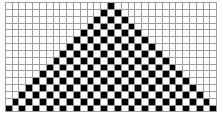
\includegraphics[]{img/wolframResult-15}
\caption{Result automata}
\end{figure}

This gives the result in figure 2. In this case the result is very well structured and organized. Wolfram discovered that there are 256 of these simple sets of rules, based on eight individual rules. Not every one of these 256 sets gives nicely structured results.

\paragraph{Music}

Wolfram used his automata to create music. Let's say we used one of the 256 sets of rules to create a result pattern. We can take a swatch through this pattern of 15 cells wide. When we flip it on its side we can treat it as a musical score.
Figure 3 shows the swath from a resulting pattern and figure 4 shows this swath as a musical score.

 \begin{figure}[h]
\centering
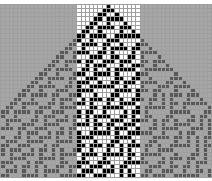
\includegraphics[]{img/wolframMusic1}
\caption{Swath through pattern}
\end{figure}

\begin{figure}[h]
\centering
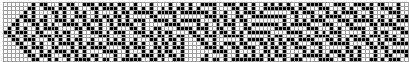
\includegraphics[]{img/wolframMusic2}
\caption{Musical score}
\end{figure}

Now we can assume that time runs across the page from left to right and every black cell represents a note played. Wolfram has developed his own language and uses various of his own algorithms to form music out of these cellular automaton patterns.
\newline
\newline
The number of rules isn't limited by eight individual rules. We can determine the color of the next cell by looking at his five upper row neighbours, instead of three. This gives a much bigger number of results (around 4 billion) and much more interesting results to use in the music creation. 

\end{document}